% abtex2-modelo-artigo.tex, v-1.9.2 laurocesar
% Copyright 2012-2014 by abnTeX2 group at http://abntex2.googlecode.com/ 
%

% ------------------------------------------------------------------------
% ------------------------------------------------------------------------
% abnTeX2: Modelo de Artigo Acadêmico em conformidade com
% ABNT NBR 6022:2003: Informação e documentação - Artigo em publicação 
% periódica científica impressa - Apresentação
% ------------------------------------------------------------------------
% ------------------------------------------------------------------------

\documentclass[
	% -- opções da classe memoir --
	article,			% indica que é um artigo acadêmico
	11pt,				% tamanho da fonte
	oneside,			% para impressão apenas no verso. Oposto a twoside
	a4paper,			% tamanho do papel. 
	% -- opções da classe abntex2 --
	%chapter=TITLE,		% títulos de capítulos convertidos em letras maiúsculas
	%section=TITLE,		% títulos de seções convertidos em letras maiúsculas
	%subsection=TITLE,	% títulos de subseções convertidos em letras maiúsculas
	%subsubsection=TITLE % títulos de subsubseções convertidos em letras maiúsculas
	% -- opções do pacote babel --
	brazil,				% o último idioma é o principal do documento
        english,			% idioma adicional para hifenização
	sumario=tradicional
	]{abntex2}

\usepackage{float}
\usepackage{lmodern}			% Usa a fonte Latin Modern
\usepackage[T1]{fontenc}		% Selecao de codigos de fonte.
\usepackage[utf8]{inputenc}		% Codificacao do documento (conversão automática dos acentos)
\usepackage{indentfirst}		% Indenta o primeiro parágrafo de cada seção.
\usepackage{nomencl} 			% Lista de simbolos
\usepackage{color}				% Controle das cores
\usepackage{graphicx}			% Inclusão de gráficos
\usepackage{microtype} 			% para melhorias de justificação
\usepackage{lipsum}				% para geração de dummy text
\usepackage[brazilian,hyperpageref]{backref}	 % Paginas com as citações na bibl
\usepackage[alf]{abntex2cite}	% Citações padrão ABNT
\renewcommand{\backrefpagesname}{Citado na(s) página(s):~}
\renewcommand{\backref}{}
\renewcommand*{\backrefalt}[4]{
	\ifcase #1 %
		Nenhuma citação no texto.%
	\or
		Citado na página #2.%
	\else
		Citado #1 vezes nas páginas #2.%
	\fi}%

\titulo{Improving the performance of a RISC-V processor for specific programs}
\autor{William Maas}
\local{Brasil}
\data{2023, September}

\definecolor{blue}{RGB}{41,5,195}
\makeatletter
\hypersetup{
     	%pagebackref=true,
		pdftitle={\@title}, 
		pdfauthor={\@author},
    	pdfsubject={Modelo de artigo científico com abnTeX2},
	    pdfcreator={LaTeX with abnTeX2},
		pdfkeywords={abnt}{latex}{abntex}{abntex2}{atigo científico}, 
		colorlinks=true,       		% false: boxed links; true: colored links
    	linkcolor=blue,          	% color of internal links
    	citecolor=blue,        		% color of links to bibliography
    	filecolor=magenta,      		% color of file links
		urlcolor=blue,
		bookmarksdepth=4
}
\makeatother
\makeindex
\setlrmarginsandblock{3cm}{3cm}{*}
\setulmarginsandblock{3cm}{3cm}{*}
\checkandfixthelayout
\setlength{\parindent}{1.3cm}
\setlength{\parskip}{0.2cm}  % tente também \onelineskip
\SingleSpacing

\begin{document}
\frenchspacing
\maketitle

\begin{abstract}
Today in the world of cutting-edge processor optimization, the marriage of innovation and specificity paves the way for unprecedented performance gains. In the context of computer architecture, the RISC-V processor has emerged as a versatile and open-source platform, bringing the attention of researchers and developers alike. However, as programs become increasingly intricate and varied, the need to tailor processors to serve specific applications has become more apparent. This article dives into the task of enhancing RISC-V processor performance for specific programs, by deeply analyzing their behavior at runtime, and turning ideas into optimization strategies.

\vspace{\onelineskip}
 
 \noindent
 \textbf{Keywords}: risc-v, gem5, cpu, programs, matrix multiplication, linked-list, breadth-first search.
\end{abstract}

\textual
\section*{Introduction}
In this research, we are going to explore the problem of optimizing the runtime performance of specific programs for a RISC-V CPU \cite{riscv-pt-wikipedia}, in order to do that we will need some tools to help simulate the programs, collect data, analyze the results, and validate the optimization hypotheses that we will propose. The end goal is to create a RISC-V CPU that is faster than the base model and/or costs less money. Our methodology revolves around a quantitative approach, where we collect data from simulations, propose optimization strategies, and analyze the outcomes.

At the core of our research is the Gem5 simulator, a powerful and versatile tool that accommodates advanced features to support fine-grained optimization of CPU models. With a base CPU model and a RISC-V architecture, we explore the intricacies of the chosen programs: Matrix multiplication (MxM), Linked List traversal (LL), and Graph Breadth-First Search (BFS). Where each has different runtime characteristics, and demands distinct CPU requirements.

Our optimization journey begins with cache optimization, recognizing the pivotal role that caches play in modern processors. Where we explore L1 instruction and data cache sizes, and the addition of an L2 cache, where we evaluate its impact on overall performance for each program.

Not stopping at caches, we go a step further into the aspect of CPU execution unit tweaks, aiming to harness instruction-level parallelism (ILP). By enhancing various hardware parameters, such as Integer Functional Units (FUs) and execution buffers, we elevate raw processing power, looking for the CPU's ability to execute multiple instructions concurrently.

The results obtained, spanning cache optimization and CPU execution unit enhancements, are documented and presented in this article. Through detailed analysis, we walk through the implications of cache size adjustments, the complexities of L2 cache integration, and the benefits of fine-tuning the CPU's execution unit.


\section{Methods}
The methodology chosen for this research was quantitative, where we defined a structured way to collect data, proposed some optimization strategies, and analyzed the results. The tooling used and the structure of the experiments are explained in the following sections. The tooling used and the simulation scripts can be found in this \href{https://github.com/wbmaas/riscv-opt}{GitHub repository} \cite{riscv-opt}.
 
\subsection{Gem5 simulator}
The gem5 simulator is a versatile platform utilized for advanced research in computer-system architecture, encompassing both system-level architecture and processor microarchitecture. Gem5 has several key features, including the availability of multiple interchangeable CPU models such as simple one-CPI, in-order, out-of-order, and KVM-based CPUs. Its event-driven memory system encompasses caches, snoop filters, and DRAM controllers, and accommodates diverse memory types, allowing flexible arrangements to model complex cache hierarchies with heterogeneous memories. The simulator offers support for multiple instruction set architectures (ISAs) like Alpha, ARM, SPARC, MIPS, POWER, RISC-V, and x86, facilitating effective ISA decoupling from CPU models. This enables gem5 to support a range of guest platforms on various host platforms. Gem5 also accommodates homogeneous and heterogeneous multi-core systems with customizable topologies and employs cache coherence protocols for maintaining cache consistency. It possesses full-system capability for ARM, x86, RISC-V, and SPARC architectures, supporting booting of Linux, Android, and other operating systems. Additionally, gem5 operates in application-only mode, executing architecture/OS binaries through Linux emulation \cite{gem5}. Based on all these characteristics we chose the Gem5 simulator to use on this research.

\subsection{MinorCPU model}
Within the Gem5 simulator, we also need to define a base CPU model to base our work on. Lucky for us, Gem5 has one that is well designed for the kind of experimentation we plan to do perform, the MinorCPU which was chosen for this project.
The Gem5's Minor CPU model is an in-order processor model with a fixed pipeline but configurable data structures and execution behavior. It is intended to be used to model processors with strict in-order execution behavior and allows visualization of an instruction’s position in the pipeline through the minorview tool. The intention is to provide a framework for micro-architecturally correlating the model with a particular, chosen processor with similar capabilities. More details about the Minor CPU architecture can be found at the \href{https://www.gem5.org/documentation/general_docs/cpu_models/minor_cpu}{Gem5 website}. The specific hardware details for the base model are the following:
\begin{itemize}
    \item Architecture: RISC-V
    \item CPU model: MinorCPU
    \item Clock speed: 2Ghz
    \item RAM: 1x 512Mb DDR3 1600Mhz
    \item L1 ICache: 32k
    \item L1 DCache: 32k
    \item L2 Cache: N/A
\end{itemize}

\subsection{Programs}
The three programs that we are going to try to optimize are Matrix multiplication (MxM), Linked List traversal (LL), and Graph Breadth-First Search (BFS). These programs were chosen because each one has different characteristics when it comes to CPU needs. The source code for the programs will be written in the C language and cross-compiled to RISC-V binaries using a cross-compilation tool. In order to perform exploratory tests and come up with some performance optimization hypotheses, we structured our programs and input datasets in a scalar way, where the input data for the programs were divided into four sets (small, medium, large, very large) for each program, and each dataset had a significant increase in size (and consequentially execution time). The input datasets used for each program are the following:

\begin{itemize}
    \item MxM size: 32x32 (small), 64x64 (medium), 128x128 (large),  256x256 (very large)
    \item LL number of nodes: 1k (small), 10k (medium), 100k (large), 300k (very large)
    \item BFS number of vertices: 64 (small), 128 (medium), 256 (large), 512 (very large)
\end{itemize}

\subsection{Optimization strategies}
It is generally known that Caches play a pivotal role in modern processors by bridging the speed gap between the fast CPU and the relatively slower main RAM memory, and they are essential for improving overall system performance and efficiency. Based on that, the first optimization strategy is to optimize the L1 instruction and data cache sizes and experiment with adding an L2 cache. Another characteristic of modern general-purpose CPUs is that they can explore ILP (instruction level parallelism) on any program during the execution time, so the second hypothesis is to try and explore ILP on the three specific programs and tweak the CPU execution unit towards their specificity. Summarizing, here are the chosen optimization strategies:
\begin{itemize}
    \item Optimize L1 instruction and data cache sizes.
    \item Adding an L2 cache.
    \item Tweak the CPU execution unit to explore ILP on the specific programs.
\end{itemize}

\section{Results}
The results obtained for the three proposed optimization strategies are described in detail in this section.

\subsection{Base CPU performance stats}
To start we collected metrics for the simulation of all programs with their dataset variations, so we can better understand the runtime behavior of the programs, and propose some hypotheses. Gem5 gives us a large number of statistics about the CPU behavior during the execution, but for this research, we choose to look at the stats that matter the most for our end goal which are the simulation seconds and cycles per instruction. In the charts from figures \ref{fig:base-cpu-mxm}, \ref{fig:base-cpu-ll} and \ref{fig:base-cpu-bfs}, we can see the execution time for the programs running on the Base CPU model.

\begin{figure}[H]
\caption{Base CPU stats - MxM}
\label{fig:base-cpu-mxm}
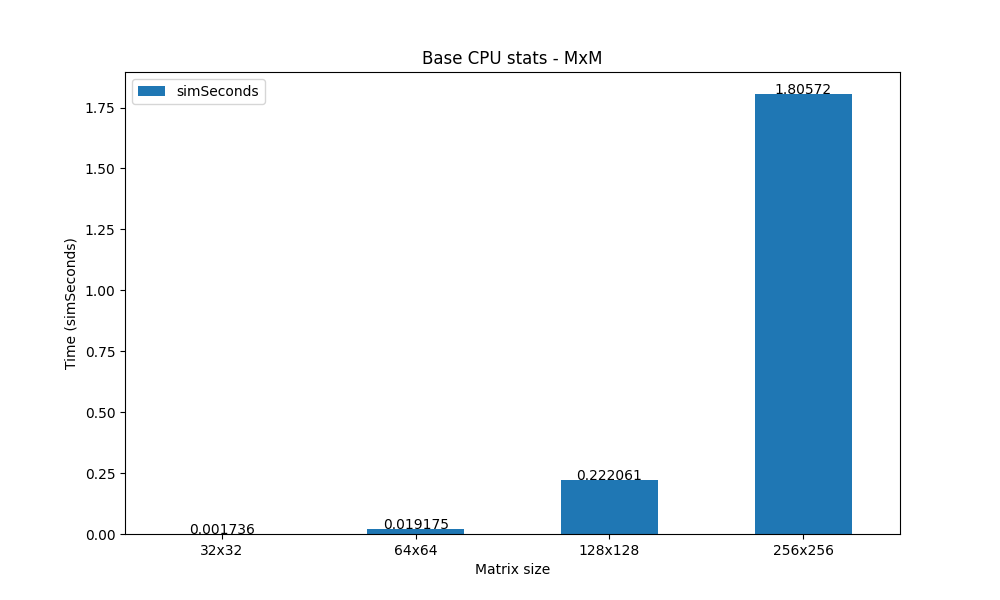
\includegraphics[width=\textwidth]{images/base-cpu-mxm.png}
\end{figure}

\begin{figure}[H]
\caption{Base CPU stats - Linked List}
\label{fig:base-cpu-ll}
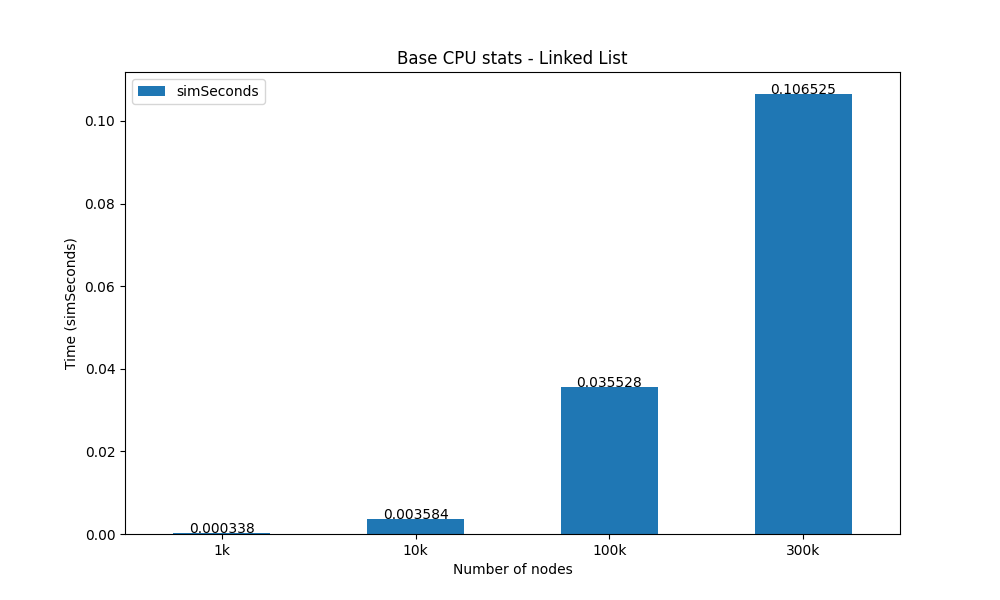
\includegraphics[width=\textwidth]{images/base-cpu-ll.png}
\end{figure}

\begin{figure}[H]
\caption{Base CPU stats - BFS}
\label{fig:base-cpu-bfs}
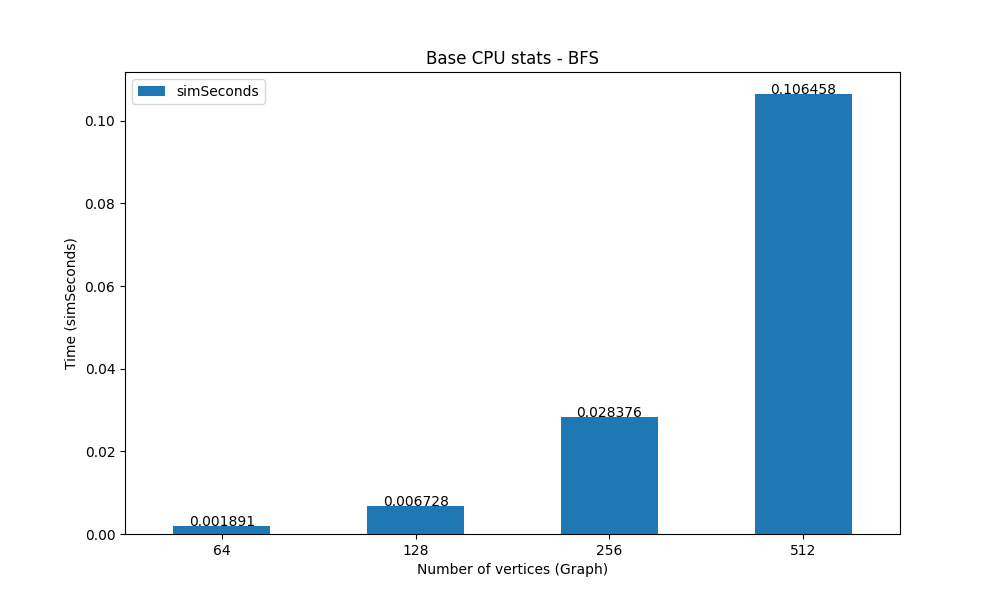
\includegraphics[width=\textwidth]{images/base-cpu-bfs.png}
\end{figure}

\subsection{Optimize L1 instruction and data cache sizes}
The first strategy is to optimize the L1 cache sizes and validate if there are any performance gains that can be obtained. The base CPU has a 32k instruction cache and a 32k data cache, we performed tests with instruction cache sizes of 8k/16k/32k/64k, combining with data caches of 32k/64k/128k for all programs and the input data variants. In the charts from figures \ref{fig:caches-mxm}, \ref{fig:caches-ll} and \ref{fig:caches-bfs}, we can see the execution time for the programs running on each L1 cache variant.

\begin{figure}[H]
\caption{L1 caches - MxM}
\label{fig:caches-mxm}
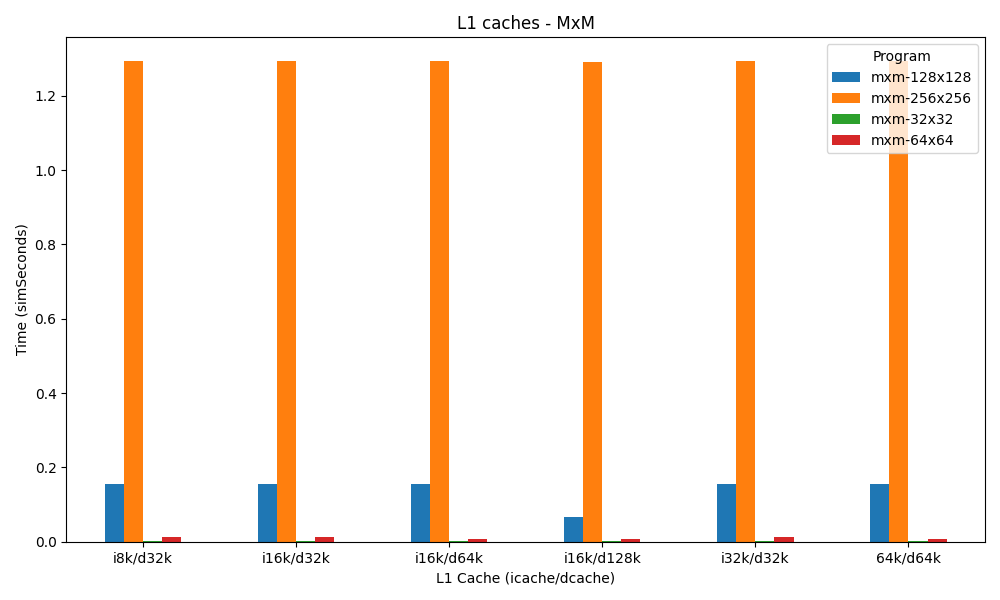
\includegraphics[width=\textwidth]{images/caches-mxm.png}
\end{figure}

\begin{figure}[H]
\caption{L1 caches - Linked List}
\label{fig:caches-ll}
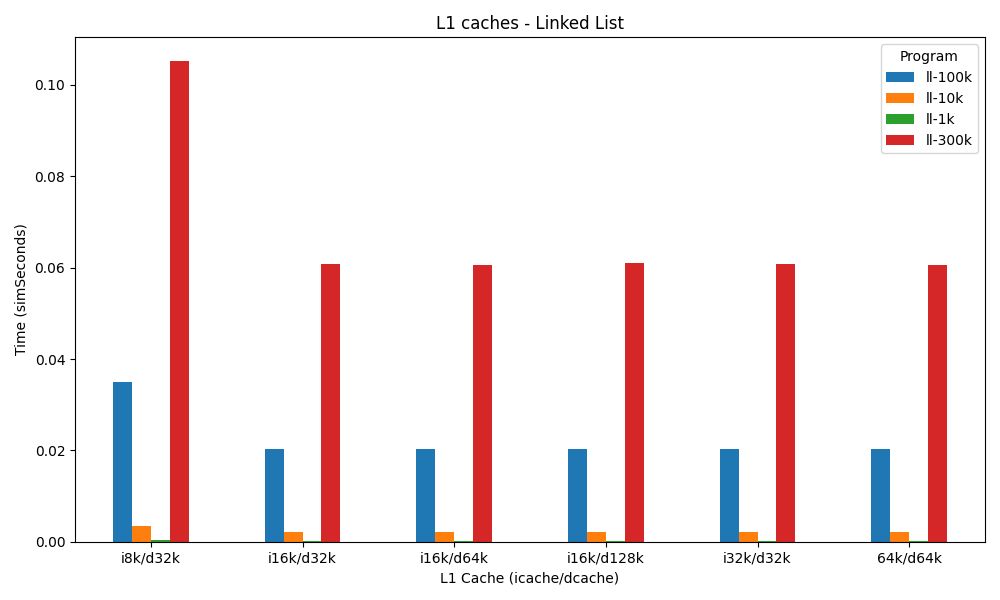
\includegraphics[width=\textwidth]{images/caches-ll.png}
\end{figure}

\begin{figure}[H]
\caption{L1 caches - BFS}
\label{fig:caches-bfs}
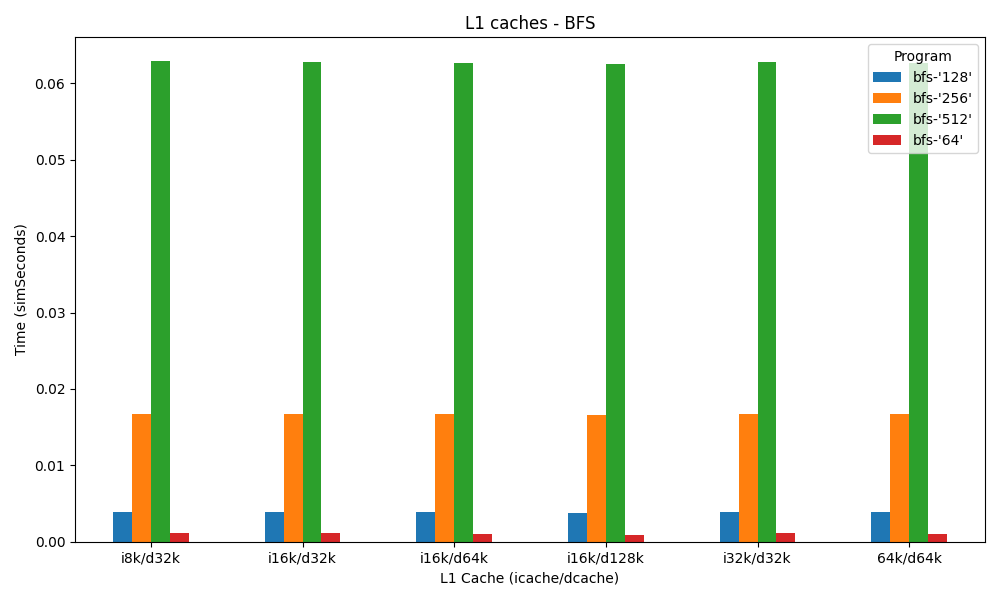
\includegraphics[width=\textwidth]{images/caches-bfs.png}
\end{figure}

With the results obtained, we can observe the following:
\begin{itemize}
    \item Instruction cache adds value up until 16k, after that, there were no performance gains for all programs.
    \item Data cache greater than 32k doesn't provide performance gains to the LL and BFS programs.
    \item A MxM of size 128x128 has a performance gain from a data cache of 128k.
    \item The MxM program reaches its peak performance for large matrices (128x128 plus) with a data cache of 32k.
\end{itemize}

Based on this analysis we can say that a L1 instruction and data cache of 16k/32k is the optimal choice with performance and cost in mind.

\subsection{Adding an L2 cache}
Based on the same principle of the L1 caches, we analyzed the performance of the CPU after adding an L2 cache of different sizes. For the test, we used the optimal L1 cache combination of 16k/32k and some other variations (16k/64k and 16k/128k which also had a good performance), in combination with an L2 cache of sizes 128k and 256k. With the results obtained, we could observe the following:
\begin{itemize}
    \item The L2 cache had a small performance improvement in a `small` MxM.
    \item The L2 cache made the performance of MxM greater than `small` worse.
    \item The L2 cache made the performance of LL worse.
    \item The L2 cache made the performance of BFS worse.
\end{itemize}
With this, we can conclude that adding an L2 Cache did not improve the performance of the programs.

\subsection{CPU execution unit tweaks}
After the cache optimization, the strategy to speed up the base CPU model even further is by adding more raw processing power. There are a lot of ways of doing that, but ideally, we need to find the right balance between instruction fetching and decoding capacity, execution buffers, logic and arithmetic FUs (Functional Units), memory I/O capacity, and so on. After performing exploratory tests with different sets of hardware additions and tweaks, we could find some optimal configurations, which are the following.
\begin{itemize}
    \item Adding more Integer FUs (2 -> 4).
    \item Increasing the instruction decode buffer (2 -> 12).
    \item Increasing the execution unit buffer (2 -> 6).
    \item Increasing the execution issue limit (2 -> 4).
    \item Increasing the capacity to read/write from memory from (2 -> 4).
\end{itemize}
In the charts from figures \ref{fig:exec-opt-mxm}, \ref{fig:exec-opt-ll} and \ref{fig:exec-opt-bfs}, we can see the execution time for the programs running on the optimized CPU model.

\begin{figure}[H]
\caption{Execution unit optimizations - MxM}
\label{fig:exec-opt-mxm}
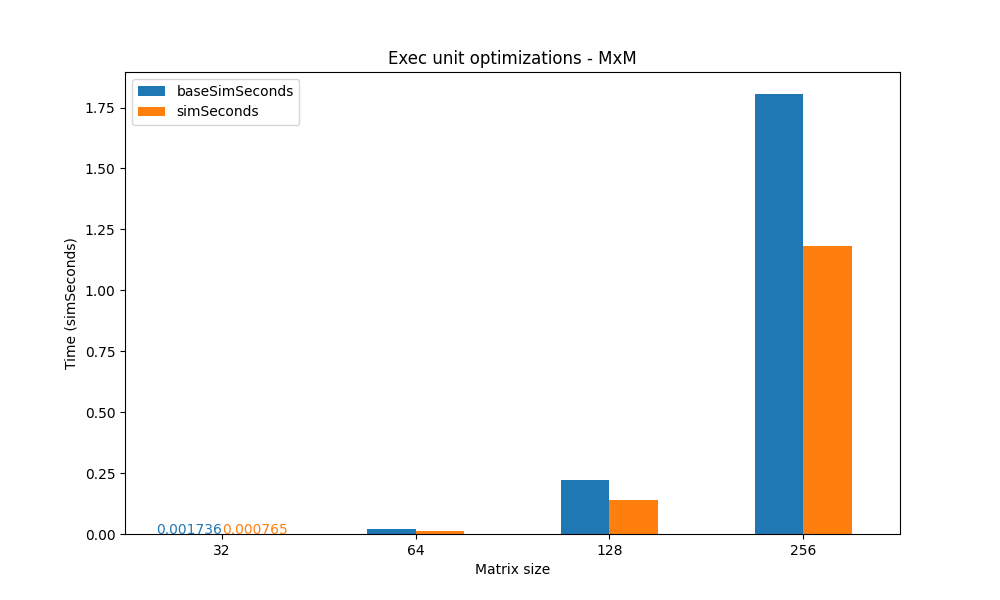
\includegraphics[width=\textwidth]{images/exec-opt-mxm.png}
\end{figure}

\begin{figure}[H]
\caption{Execution unit optimizations - Linked List}
\label{fig:exec-opt-ll}
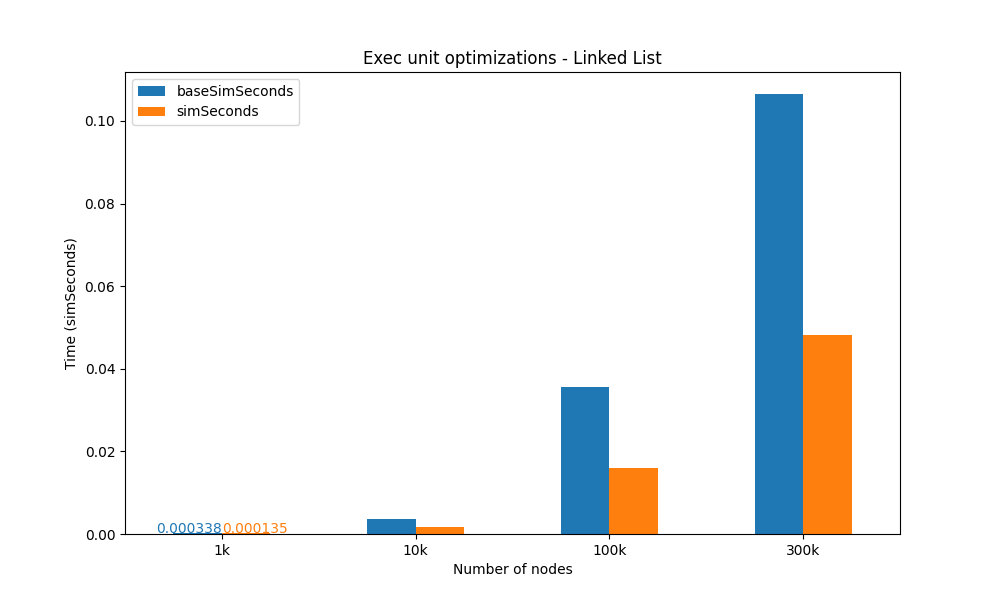
\includegraphics[width=\textwidth]{images/exec-opt-ll.png}
\end{figure}

\begin{figure}[H]
\caption{Execution unit optimizations - BFS}
\label{fig:exec-opt-bfs}
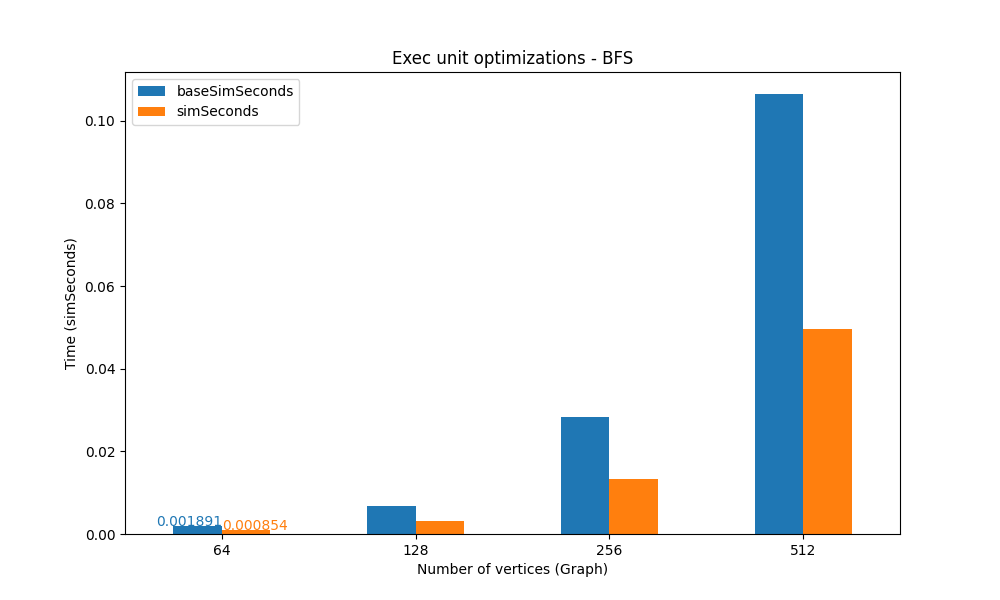
\includegraphics[width=\textwidth]{images/exec-opt-bfs.png}
\end{figure}

By analyzing the data, we can observe performance gains in all three programs, and for all input sizes. Between the MxM, Linked List, and BFS, we got on average a 2.18x speed up. The speed up gain for each program and input size combination is shown in table \ref{table:speedup}.

\begin{table}[]
\caption{Programs speed up}
\label{table:speedup}
\begin{tabular}{|lr|r|r|l}
\cline{1-4}
\multicolumn{1}{|l|}{\textbf{Program}} & \multicolumn{1}{c|}{\textbf{Base CPU}} & \multicolumn{1}{c|}{\textbf{Optimized CPU}} & \multicolumn{1}{c|}{\textbf{Speed up}} &  \\ \cline{1-4}
\multicolumn{1}{|l|}{MxM 32x32}        & 0.0017                                 & 0.0007                                      & 2.26x                                  &  \\ \cline{1-4}
\multicolumn{1}{|l|}{MxM 64x64}        & 0.0191                                 & 0.0105                                      & 1.81x                                  &  \\ \cline{1-4}
\multicolumn{1}{|l|}{MxM 128x128}      & 0.2220                                 & 0.1413                                      & 1.57x                                  &  \\ \cline{1-4}
\multicolumn{1}{|l|}{MxM 256x256}      & 1.8057                                 & 1.1830                                      & 1.52x                                  &  \\ \cline{1-4}
\multicolumn{1}{|l|}{LL 1k}            & 0.0003                                 & 0.0001                                      & 2.50x                                  &  \\ \cline{1-4}
\multicolumn{1}{|l|}{LL 10k}           & 0.0035                                 & 0.0016                                      & 2.20x                                  &  \\ \cline{1-4}
\multicolumn{1}{|l|}{LL 100k}          & 0.0355                                 & 0.0160                                      & 2.21x                                  &  \\ \cline{1-4}
\multicolumn{1}{|l|}{LL 300k}          & 0.1065                                 & 0.0481                                      & 2.21x                                  &  \\ \cline{1-4}
\multicolumn{1}{|l|}{BFS 64}           & 0.0018                                 & 0.0008                                      & 2.21x                                  &  \\ \cline{1-4}
\multicolumn{1}{|l|}{BFS 128}          & 0.0067                                 & 0.0031                                      & 2.17x                                  &  \\ \cline{1-4}
\multicolumn{1}{|l|}{BFS 256}          & 0.0283                                 & 0.01320                                     & 2.14x                                  &  \\ \cline{1-4}
\multicolumn{1}{|l|}{BFS 512}          & 0.1064                                 & 0.04969                                     & 2.14x                                  &  \\ \cline{1-4}
\multicolumn{2}{|l|}{}                                                          & Average                                     & 2.18x                                  &  \\ \cline{1-4}
\end{tabular}
\end{table}

\section{Discussion}
The pursuit of optimizing the runtime performance of specific programs for RISC-V CPUs, using the Gem5 simulator and the MinorCPU model, has led us to valuable insights and results. In this section, we delve into the implications and significance of our findings and discuss their broader implications for computer architecture and optimization.

\subsection{Cache Optimization}
Our first optimization strategy focused on adjusting the sizes of the L1 instruction and data caches and exploring the addition of an L2 cache. The results highlighted the critical role of cache size in program performance.

For the L1 caches, we observed that increasing the instruction cache size up to 16k yielded performance gains, emphasizing the importance of accommodating instruction data efficiently. However, beyond 16k, additional increases did not yield further improvements, indicating diminishing returns. In contrast, the data cache showed varying results. For the Matrix multiplication (MxM) program, larger data caches, such as 128k, led to performance improvements, especially for larger matrix sizes. However, for Linked List traversal (LL) and Graph Breadth-First Search (BFS), larger data caches did not result in significant gains. These findings suggest that cache size optimization should be tailored to the specific program's memory access patterns and requirements.

Regarding the L2 cache, our experiments did not yield consistent performance improvements. In fact, for some programs, including LL and BFS, the addition of an L2 cache led to performance degradation. These results highlight the complexity of cache hierarchies and the need for careful consideration of cache configurations based on program characteristics. A one-size-fits-all approach is insufficient, and optimizing cache hierarchies requires a program-specific focus.

\subsection{CPU Execution Unit Tweaks} 
The second optimization strategy involved enhancing the CPU execution unit to explore instruction-level parallelism (ILP) for the specific programs under study. We made adjustments to various hardware parameters within Gem5, including Integer Functional Units (FUs), instruction decode buffer, execution unit buffer, execution issue limit, and memory I/O capacity.

Our findings revealed that increasing the Integer FUs and expanding various buffer sizes led to substantial performance improvements. These enhancements effectively increased the raw processing power of the CPU, allowing it to handle multiple instructions concurrently. This approach proved effective for all three programs since we could exploit ILP. The logarithmic scale plot of simSeconds demonstrated the scalability of performance gains with different input sizes showing that the hardware extensions scaled well across various program sizes, indicating its robustness and potential for broader applicability.

\subsection{Conclusion}
In conclusion, this research's efforts have yielded valuable insights into optimizing the runtime performance of specific programs for a RISC-V CPU. Through the exploration of optimization strategies, including cache adjustments and CPU execution unit enhancements, we have achieved key factors that impact program performance. Overall, our findings underscore the importance of tailoring optimization strategies to the unique characteristics of the target programs. This research contributes to our understanding of computer architecture optimization and provides a foundation for future work in enhancing the performance of RISC-V CPUs in diverse computing environments.

\bibliography{references}



\end{document}
